%% V1.0
%% by Gabriel Garcia, gabrcg@gmail.com
%% This is a template for Udacity projects using IEEEtran.cls

%% Be Udacious!

\documentclass[10pt,journal,compsoc]{IEEEtran}

\usepackage[pdftex]{graphicx}    
\usepackage{cite}
\hyphenation{op-tical net-works semi-conduc-tor}


\begin{document}

\title{Robotic Inference: Classification Network}

\author{Hsin-Wen Chang}

\markboth{Inference project, Robotic Nanodegree, Udacity}%
{}
\IEEEtitleabstractindextext{%

\begin{abstract}
In this project,NVIDIA DIGITS workflow are used for rapidly prototype ideas that can be deployed on the Jetson
near real time. With DIGITS prototype classification networks and training a CNN on the
supplied data and train another CNN using a combination data set from the GTI vehicle image database, the KITTI vision benchmark suite, and examples extracted from the Udacity Self Driving Car Nanodegree - Vehicle Detection project video itself [7].
\end{abstract}

% Note that keywords are not normally used for peerreview papers.
\begin{IEEEkeywords}
Robotic inference, image classification, Udacity, NVIDIA DIGITS, deep learning.
\end{IEEEkeywords}}


\maketitle
\IEEEdisplaynontitleabstractindextext
\IEEEpeerreviewmaketitle
\section{Introduction}
\label{sec:introduction}

\IEEEPARstart{M}{achine} learning methods base on Deep learning neural network such as Classification Network and Detection Network achieved remarkable result in a wide variety domains. 
In this paper VGG16, AlexNet and GoogLeNet will be trained with Supplied data set and a combination data set [7][8]. 

introduction should provide some material regarding the history of the problem, why it is important and what is intended to be achieved. If there exists any previous attempts to solve this problem, this is a great place to note these while conveying the differences in your approach (if any). The intent is to provide enough information for the reader to understand why this problem is interesting and setting up the conversation for the solution you have provided
Use this space to introduce your robotic inference idea and how you wish to apply it. 
If you have any papers / sites you have referenced for your idea, please make sure to cite them.

\subsection{Supplied Data set}
Subsection text here.
%example for inserting image
\begin{figure}[thpb]
      \centering
      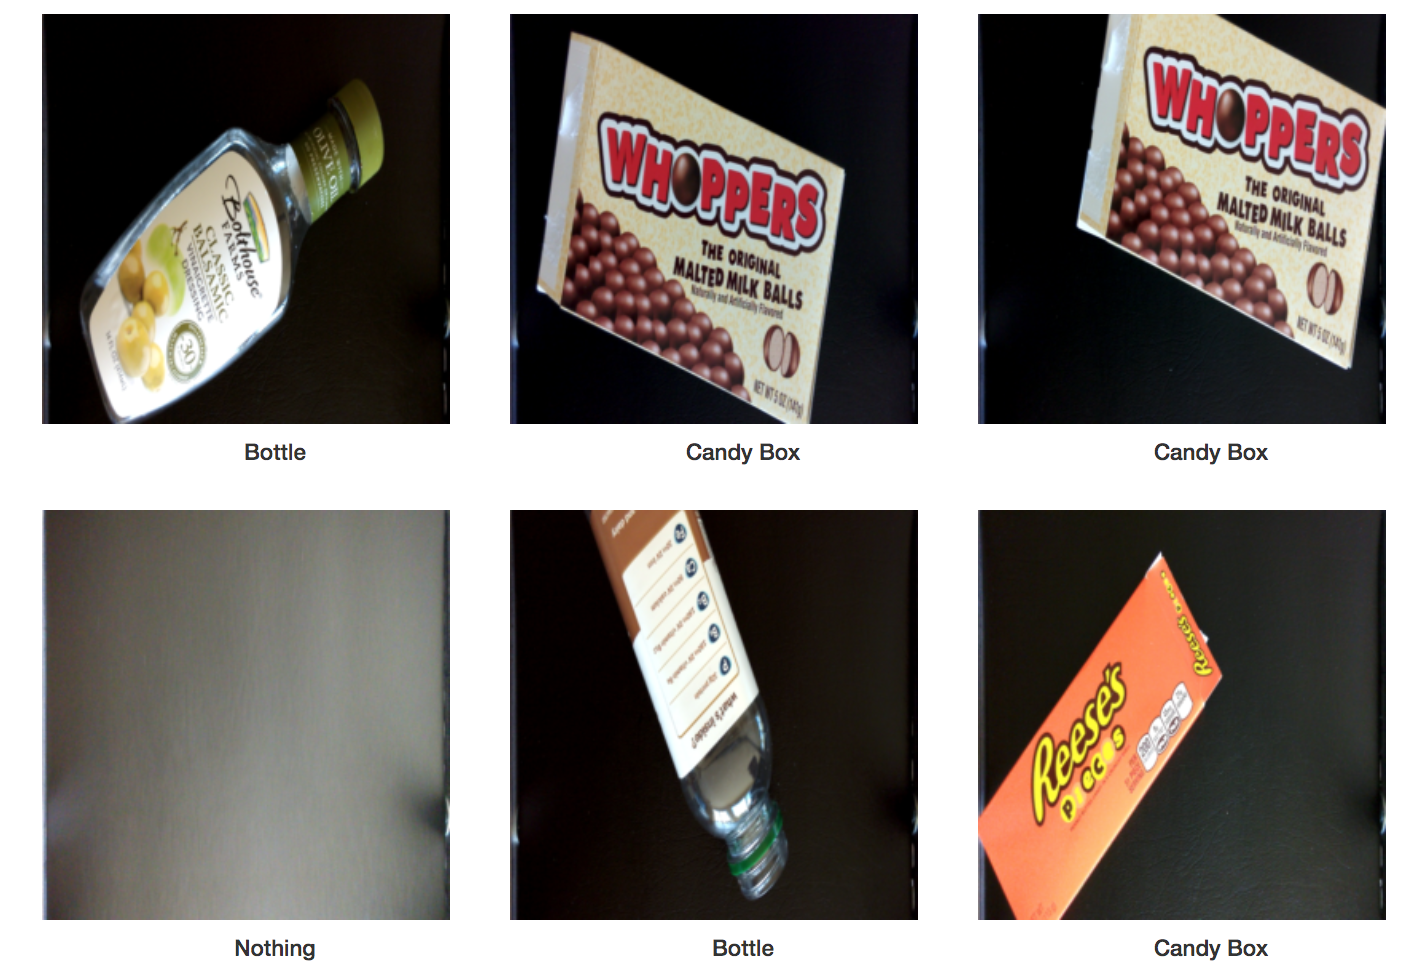
\includegraphics[width=\linewidth]{suplieDataset.png}
      \caption{Supplied Data set.}
      \label{fig:robot1}
\end{figure}
\subsubsection{Supplied Data set}
Udacity supplied dataset contain candy boxes, bottles, and nothing (empty conveyor belt).

\begin{table}[h]
 \begin{center}
      \begin{tabular}{ |c|c|c| } 
       \hline
       Class & Images & Image Shape \\
       \hline
       Candy Box & 1871 & 256x256x3 \\ 
       Bottle & 3426 & 256x256x3 \\ 
       Nothing & 2273 & 256x256x3 \\
       \hline
       Total & 7570 & \\
       \hline
      \end{tabular}
      \caption{Count of supplied data images}
      \label{table:1}
      \end{center}
      \end{table}
%example for inserting image
\begin{figure}[thpb]
      \centering
      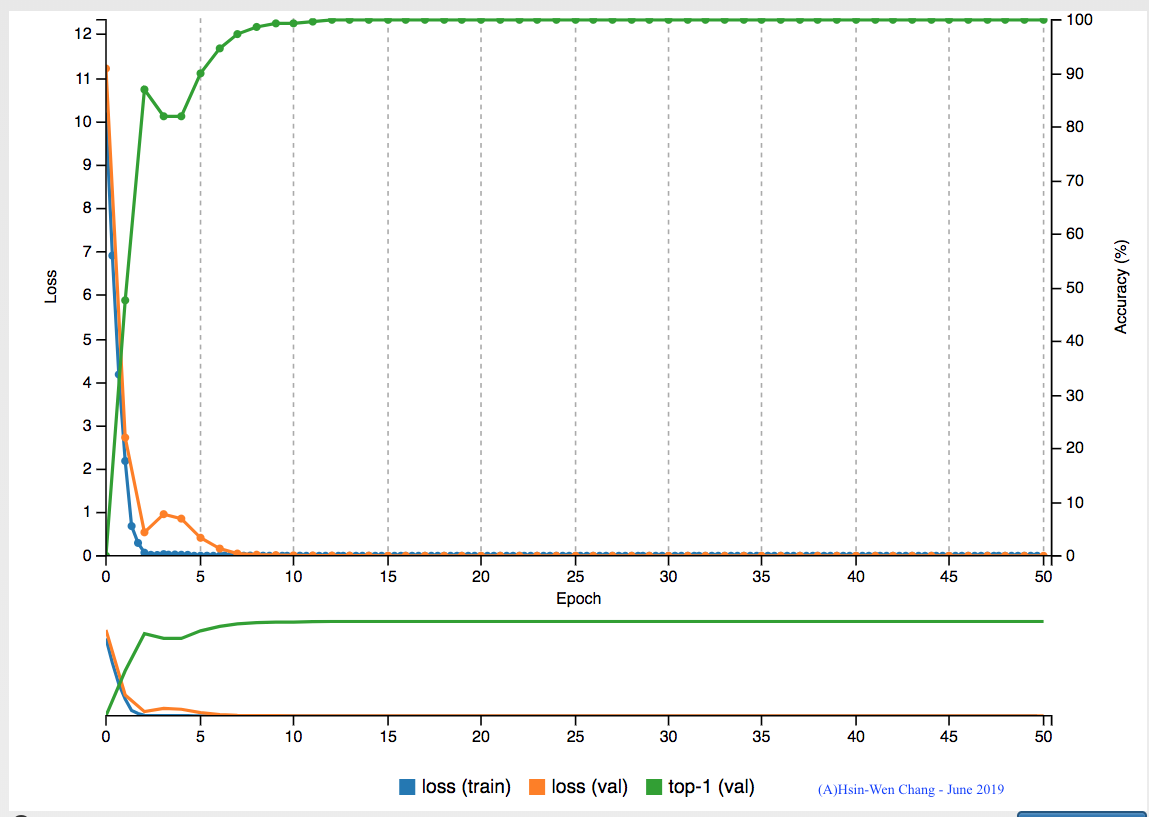
\includegraphics[width=\linewidth]{VGG16AcurracyLoss.png}
      \caption{VGG16 pretrained model}
      \label{fig:robot1}
\end{figure}
\begin{figure}[thpb]
      \centering
      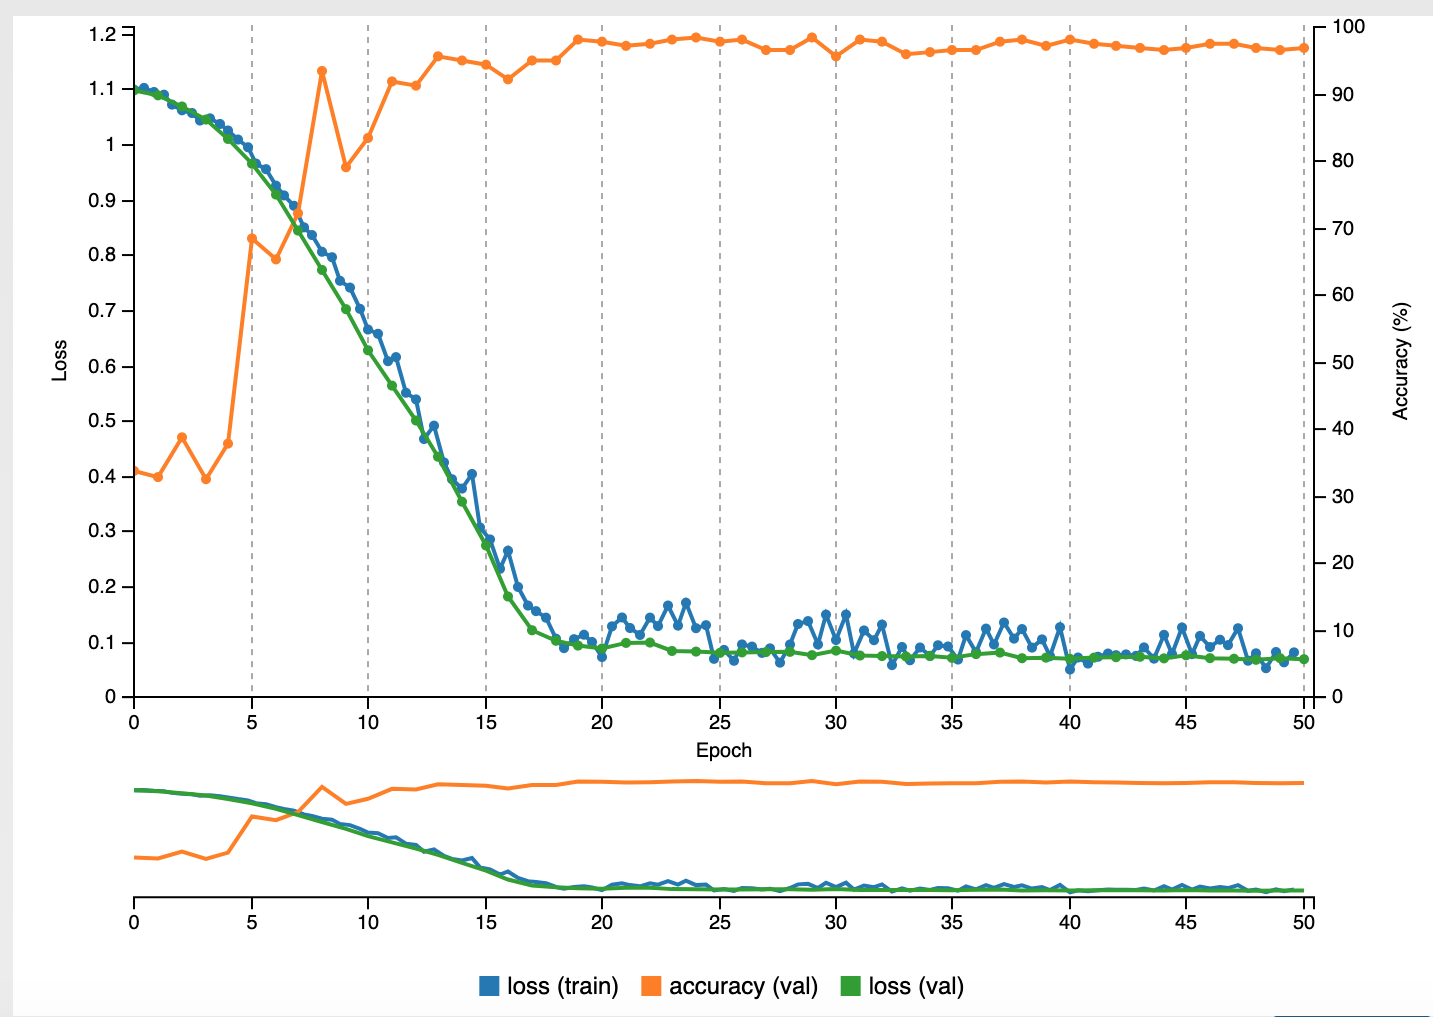
\includegraphics[width=\linewidth]{AlexNet.png}
      \caption{AlexNet}
      \label{fig:robot1}
\end{figure}
%example for inserting image
\begin{figure}[thpb]
      \centering
      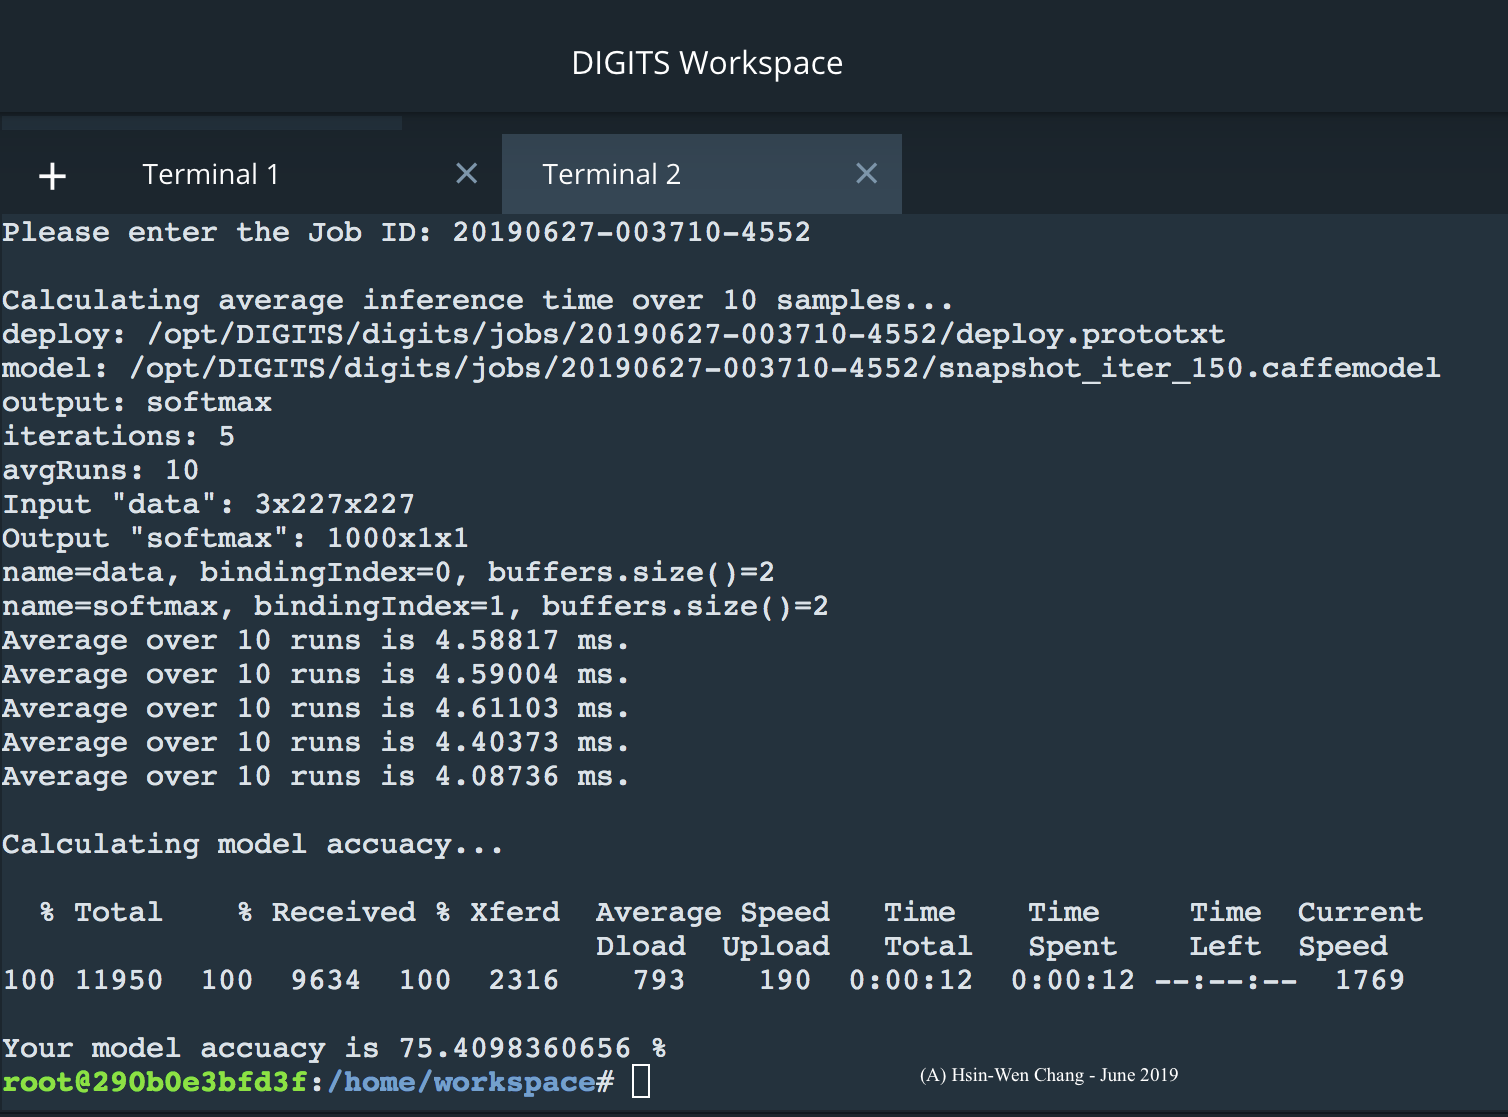
\includegraphics[width=\linewidth]{evaluate.png}
      \caption{Evaluate training result in DIGITS Workspace}
      \label{fig:robot1}
\end{figure}

\section{Background / Formulation}
%example for inserting image
\begin{figure}[thpb]
      \centering
      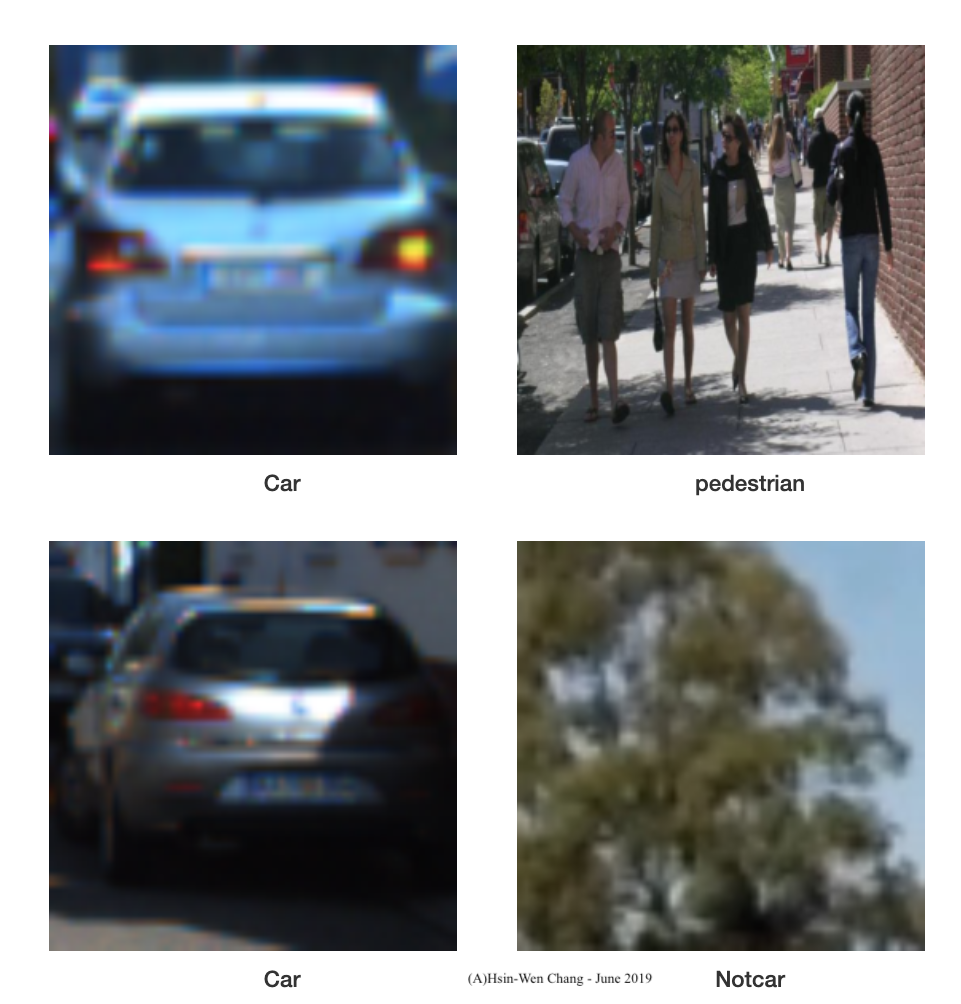
\includegraphics[width=\linewidth]{mixDataset.png}
      \caption{Combination data set.}
      \label{fig:robot1}
\end{figure}
These example images come from a combination of the GTI vehicle image database, the KITTI vision benchmark suite, and examples extracted from the project video itself. Penn-Fudan Database for Pedestrian Detection and Segmentation

 The intuition is from:
 %example for Bullet point list

\begin{itemize}
\item Can you form a model that can tell the difference between cars by type or colour?
\item Which cars are manufactured by Tesla vs BMW?
\end {itemize}
 
At this stage, you should begin diving into the technical details of your approach by explaining to the reader how parameters were defined, what type of network was chosen, and the reasons these items were performed. This should be factual and authoritative, meaning you should not use language such as “I think this will work” or “Maybe a network with this architecture is better..”. Instead, focus on items similar to, ”A 3-layer network architecture was chosen with X, Y, and Z parameters” 
Explain why you chose the network you did for the supplied data set and then why you chose the network used for your robotic inference project. \cite{lamport1994latex}

%example for Bullet point list

\begin{itemize}
\item example
\end {itemize}



%example for numbered list
\begin{enumerate}
\item example

\end{enumerate}

\section{Data Acquisition}

This section should discuss the data set. Items to include are the number of images, size of the images, the types of images (RGB, Grayscale, etc.), how these images were collected (including the method). Providing this information is critical if anyone would like to replicate your results. After all, the intent of reports such as these are to convey information and build upon ideas so you want to ensure others can validate your process.
Justifying why you gathered data in this way is a helpful point, but sometimes this may be omitted here if the problem has been stated clearly in the introduction.
It is a great idea here to have at least one or two images showing what your data looks like for the reader to visualize.

\section{Results-}
%example for inserting image
\begin{figure}[thpb]
      \centering
      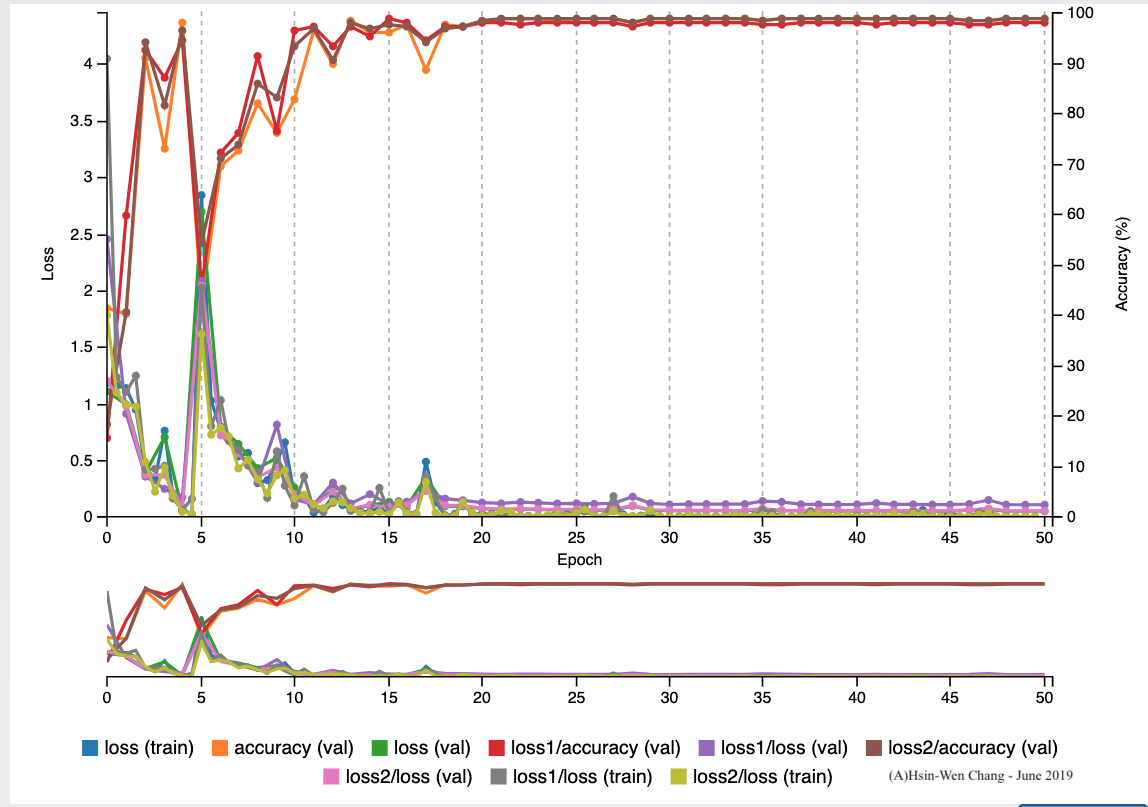
\includegraphics[width=\linewidth]{GoogLeNET.png}
      \caption{Combination data train with GoogLeNet}
      \label{fig:robot1}
\end{figure}

This is typically the hardest part of the report for many. You want to convey your results in an unbiased fashion. If you results are good, you can objectively note this. Similarly, you may do this if they are bad as well. You do not want to justify your results here with discussion; this is a topic for the next session. 
Present the results of your robotics project model and the model you used for the supplied data with the appropriate accuracy and inference time
For demonstrating your results, it is incredibly useful to have some charts, tables, and/or graphs for the reader to review. This makes ingesting the information quicker and easier.

\begin{figure}[thpb]
      \centering
      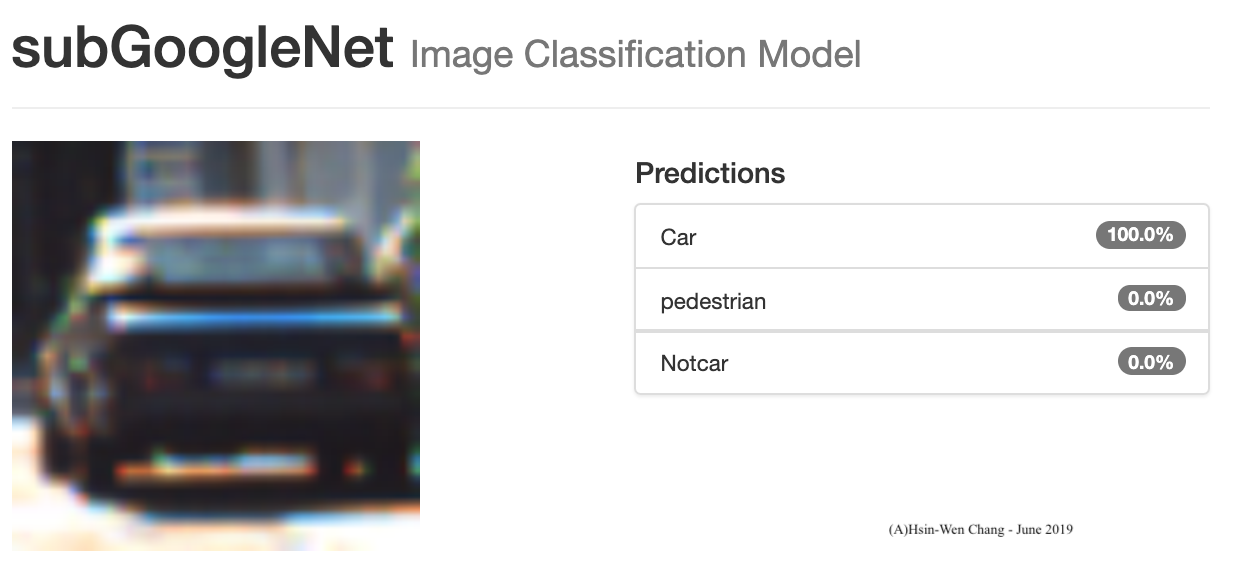
\includegraphics[width=\linewidth]{CarInferenceResult.png}
      \caption{GoogLeNet Model Inference Result: Car}
      \label{fig:robot1}
\end{figure}
\begin{figure}[thpb]
      \centering
      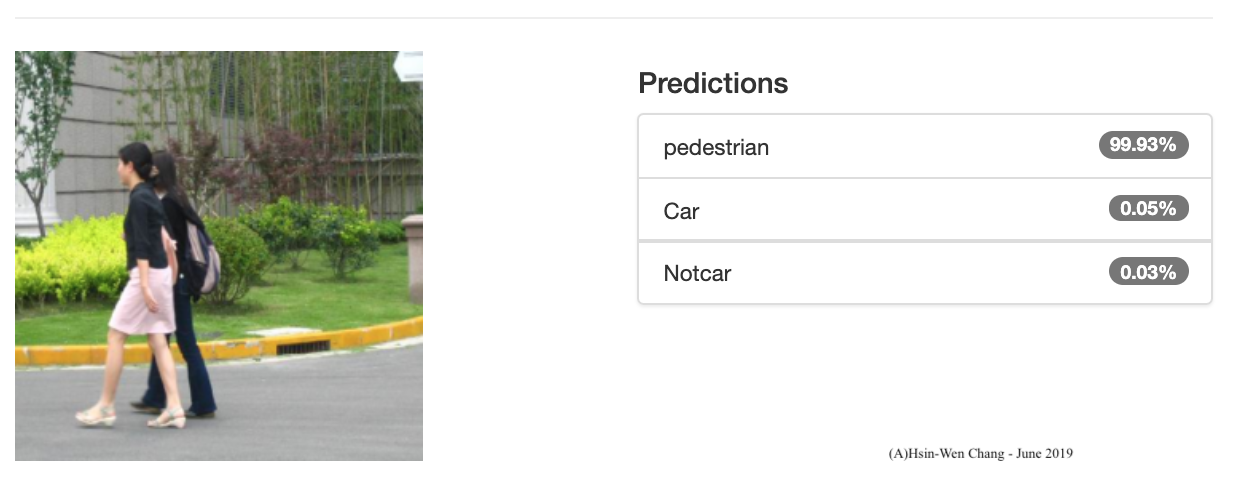
\includegraphics[width=\linewidth]{GoogLenetPed.png}
      \caption{GoogLeNet Model Inference Result: Pedestrian}
      \label{fig:robot1}
\end{figure}
\begin{figure}[thpb]
      \centering
      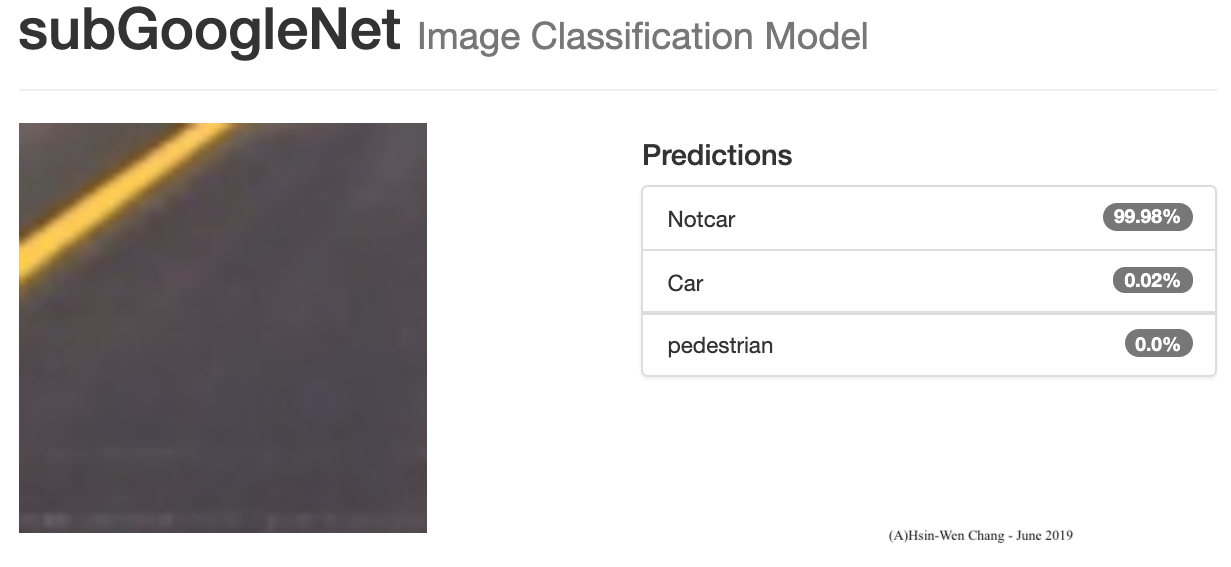
\includegraphics[width=\linewidth]{notCarInferenceGoodResult.png}
      \caption{GoogLeNet Model Inference Result: Not Car}
      \label{fig:robot1}
\end{figure}
\begin{figure}[thpb]
      \centering
      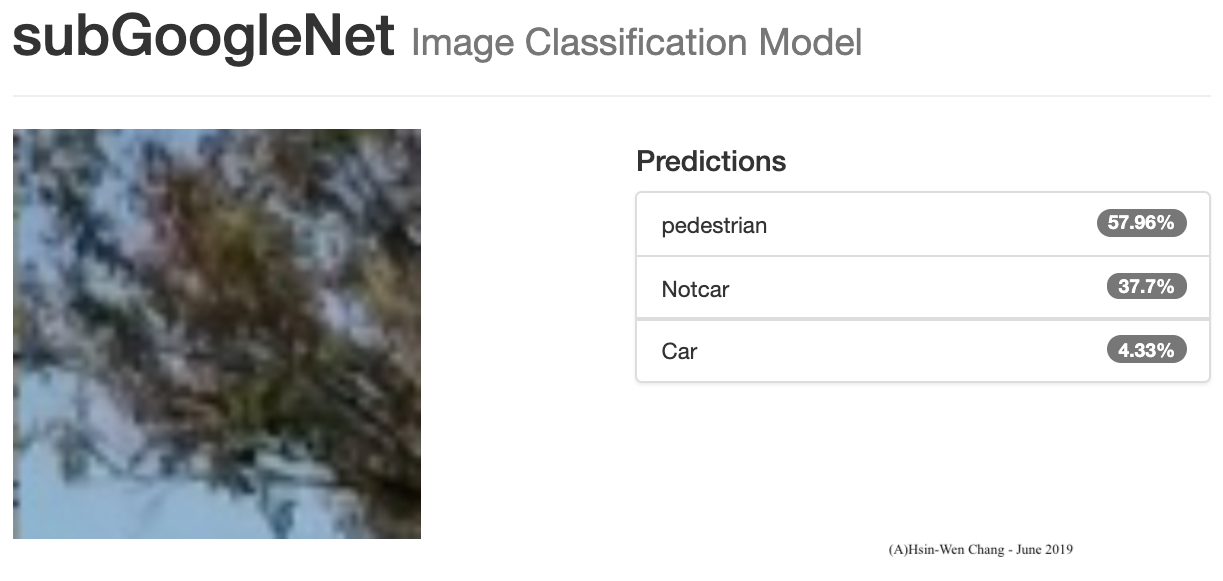
\includegraphics[width=\linewidth]{NotCarInference.png}
      \caption{GoogLeNet Model Inference Result: Not Car}
      \label{fig:robot1}
\end{figure}


\section{Discussion}
This is the only section of the report where you may include your opinion. However, make sure your opinion is based on facts. If your results are poor, make mention of what may be the underlying issues. If the results are good, why do you think this is the case? Again, avoid writing in the first person (i.e. Do not use words like “I” or “me”). If you really find yourself struggling to avoid the word “I” or “me”; sometimes, this can be avoid with the use of the word “one”. As an example: instead of : “I think the accuracy on my dataset is low because the images are too small to show the necessary detail” try: “one may believe the accuracy on the dataset is low because the images are too small to show the necessary detail”. They say the same thing, but the second avoids the first person. 
Reflect on which is more important, inference time or accuracy, in regards to your robotic inference project.

\section{Conclusion / Future work}
This section is intended to summarize your report. Your summary should include a recap of the results, did this project achieve what you attempted, and is this a commercially viable product? 
For Future work,address areas of work that you may not have addressed in your report as possible next steps. For future work, this could be due to time constraints, lack of currently developed methods / technology, and areas of application outside of your current implementation. Again, avoid the use of the first-person.

\bibliography{bib}
\bibliographystyle{ieeetr}
[2] The Caltech Database (Computational Vision at California Institute of Technology, Pasadena), http://www.vision.caltech.edu/html-files/archive.html. Accessed 14 May 2011.

[3] R Fergus, P Perona, A Zisserman, in Proceedings of the IEEE Computer Society Conference on Computer Vision and Pattern Recognition, Madison, Wisconsin, 16–22 June 2003.

[4] The TU Graz-02 Database (Graz University of Technology). Accessed 14 May 2011. 

[5] A Opelt, A Pinz, in Proceedings of the 14th Scandinavian Conference on Image Analysis, Joensuu, Finland, 19–22 June 2005.

[6] Are we ready for Autonomous Driving? The KITTI Vision Benchmark Suite, Andreas Geiger, Philip Lenz and Raquel Urtasun, Conference on Computer Vision and Pattern	Recognition (CVPR).

[7] Udacity Self-Driving car Engineer Vehicle detection project.

[8] Object Detection Combining Recognition and Segmentation. Liming Wang, Jianbo Shi, Gang Song, I-fan Shen. To Appear in ACCV 2007
\end{document}